\chapter{Method}
\label{sec:method}
As explained in \Cref{sec:introduction} the aim of this work is to find a drone
design that is the result of an optimization problem, which tends to maximize the
MAV's omni-directionality, flight efficiency and controllability. To do so it is
important to first state what are the parameters that define the design of an MAV.
These parameters are defined as:

\begin{itemize}
\item $\beta$  (angles formed by the arms with the horizontal plane see \Cref{fig:drone_design})
\item $\theta$ (angles formed by the arms in the horizontal plane see \Cref{fig:drone_design})
\item L (arm length)
\item n (number of propeller)
\end{itemize}

\begin{figure}[h]
\centering
\begin{minipage}[t]{0.3\textwidth}
  \centering
  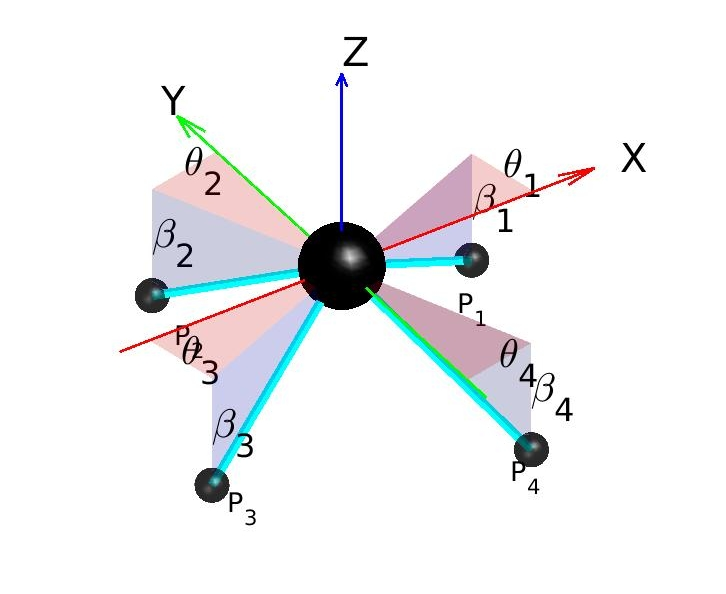
\includegraphics[width=\textwidth]{images/drone_design.jpg}
\end{minipage}
\hfill
\begin{minipage}[t]{0.3\textwidth}
  \centering
  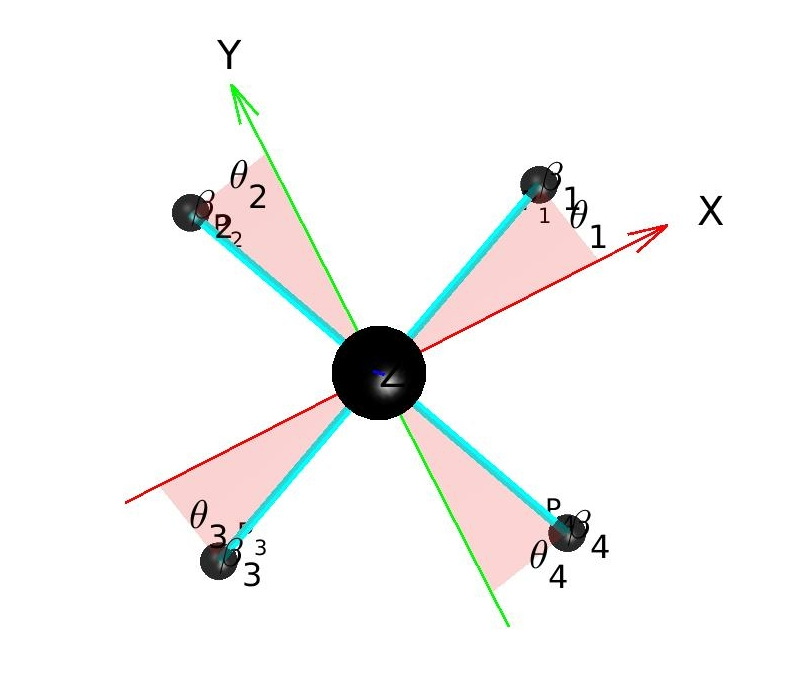
\includegraphics[width=\textwidth]{images/drone_design1.jpg}
\end{minipage}
\hfill
\begin{minipage}[t]{0.3\textwidth}
  \centering
  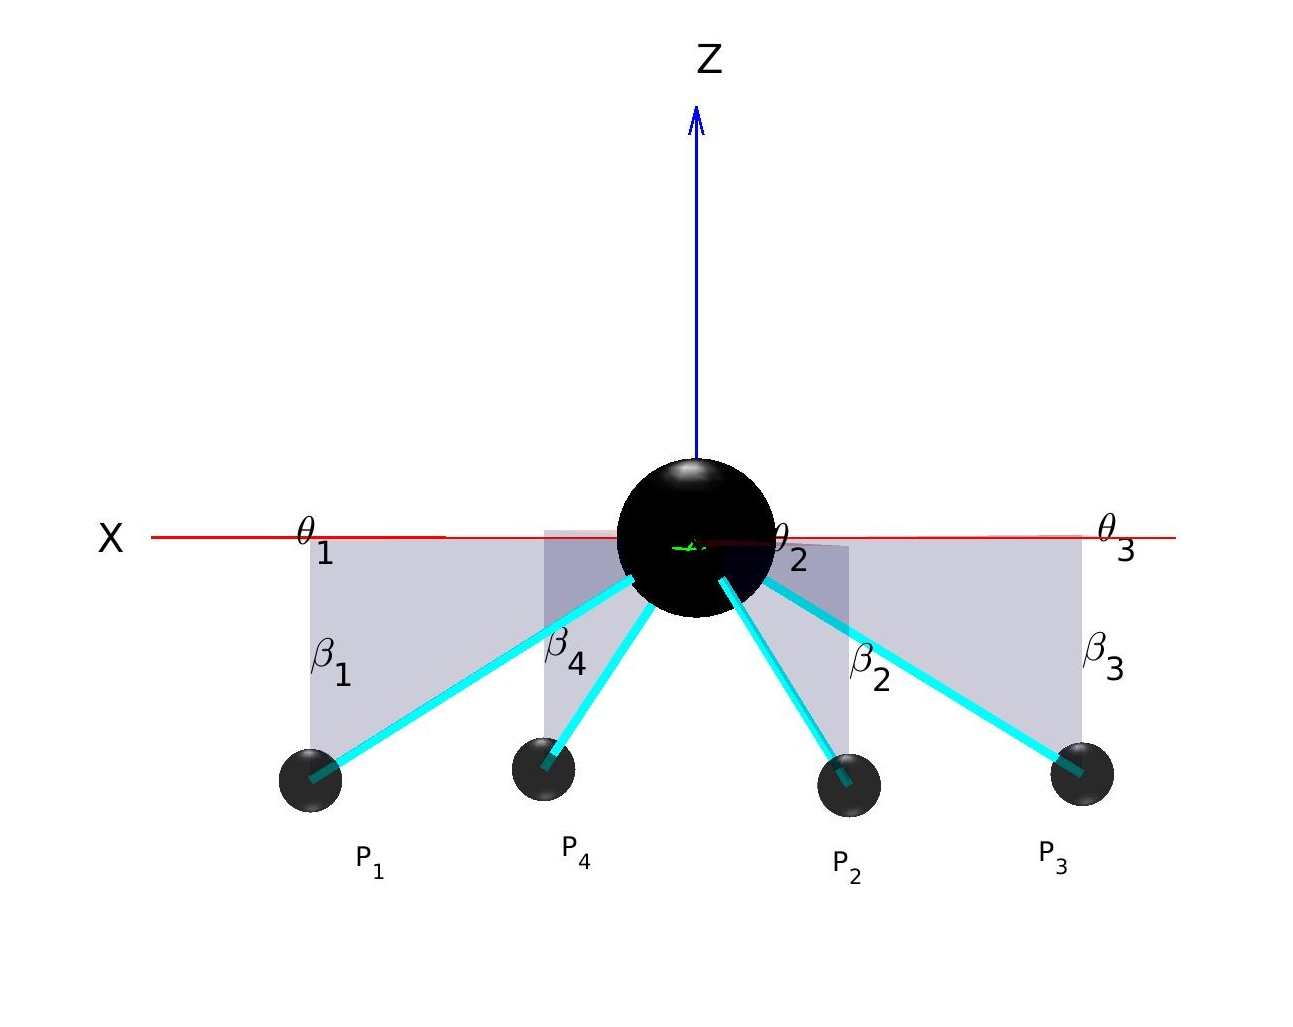
\includegraphics[width=\textwidth]{images/drone_design2.jpg}
\end{minipage}
\caption{Quadcopter to illustrate the parameters that define the morphology of an
MAV ($n = 4$, $\beta = [30, 30, 30, 30] [^{\circ}]$, $\theta = [22, 22, 22, 22]
[^{\circ}]$, and $L = 0.4 [m]$).}
\label{fig:drone_design}
\end{figure}

To solve the problem an optimization engine is developed with
Matlab$^\textrm{\textregistered}$. This tool returns the aforementioned
parameters along with other information on the corresponding MAV design.
The interesting drone designs outputted by the tool are then simulated on
Gazebo\footnote{An open source robot simulator \citep{noauthor_gazebo_nodate}.}
and the control of the different models is achieved using a Robotic Operating
System\footnote{An open source collection of software that help developers to
create robot applications \citep{rostutorials}.} (ROS) node.\\
This chapter first covers the theory needed to obtain a generalize mathematical
model for a n-rotor MAV with an arbitrary morphology. Then, the optimization
problem is defined. Afterwards, the optimization tool is described. In the end,
the theoretical background needed to perform the simulations is covered.

\section{Modelisation of MAVs}
\label{sec:modeling_mav}
In the following part, a dynamical model for a general design of MAV is presented.
Such a modelisation is much needed to mathematiacally optimize the morphology of
a MAV. This model is inspired from the models presented in
\citep{kamel_voliro:_2018} and \citep{ryll_modeling_2012}.

\subsubsection{Initial Definitions}
\label{sec:definitions}
In order to understand correctly the dynamical model, a few definitions are much
needed. First, let us define $\mathcal{F}_{W} : \{O_{W}; X_{W},  Y_{W},  Z_{W}\}$
as the world fixed inertial frame and $\mathcal{F}_{B}: \{O_{B}, X_{B},  Y_{B},
Z_{B}\}$
as a moving frame attached to the MAV. Also, $\mathcal{F}_{P_{i}} : \{O_{P_{i}};
X_{P_{i}}, Y_{P_{i}},  Z_{P_{i}}\}, i = 1...n$ is the frame of the i-th propeller.
The propeller rotate around the axis $Z_{P_{i}}$, and thus the thrust $T_{i}$ is
produced along this axis. The tilt movement of the rotors is a simple rotation
around $X_{P_{i}}$. Now let $^{W}R_{B}$ be the orientation of the body frame
with respect to the world frame and $^{B}R_{P_{i}}$ be the orientation of the
i-th propeller with respect to the body frame. From there, it
straightforward with the help of \Cref{fig:tilt_model} that

\begin{equation}
  \label{rot_b_pi}
  ^{B}R_{P_{i}} \ = \ R_{Z}\bigg((i-1)\frac{2\pi}{n}\bigg) R_Z(\theta_i)
  R_Y(\beta_i) R_{X}(\alpha_{i}),\  i = 1...n\, .
\end{equation}

Equivalently, let

\begin{equation}
  \label{O_pi}
  ^{B}O_{P_{i}} \ = \ R_{Z}\bigg((i-1)\frac{2\pi}{n}\bigg) R_Z(\theta_i) R_Y(\beta_i)
  \begin{bmatrix}
    L \\
    0 \\
    0
  \end{bmatrix}
  ,\   i = 1...n \,
\end{equation}

be the origin of the i-th propeller frame  $\mathcal{F}_{P_{i}}$.
In \Cref{rot_b_pi} and (\ref{O_pi}), $(i-1)\frac{2\pi}{n}$ is the angle that
the i-th arm would form with axis $X_B$ if the arms of the drone are evenly
distributed in the horizontal plane, $\theta_i$ is the angle that i-th arm forms
in the horizontal plane with respect to its evenly distributed position
(see \Cref{fig:drone_design}), $\beta_i$ is the angle that the i-th arm forms with
the horizontal plane (see \Cref{fig:drone_design}), $\alpha_{i}$ is the tilting
angles of the i-th propeller about the $X_{P_{i}}$ axis, L is the arm length and
n is the number of propellers.

\begin{figure}[h]
  \centering
  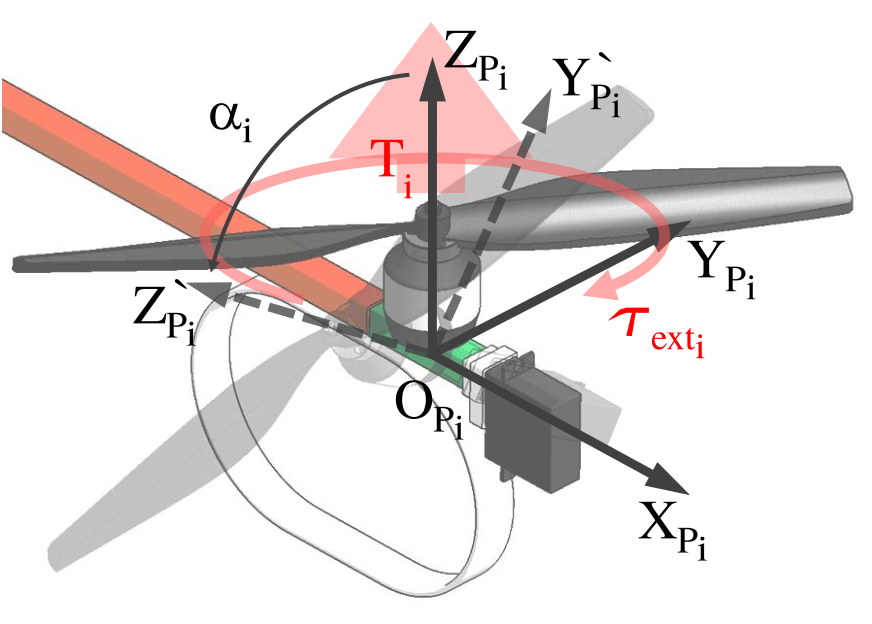
\includegraphics[width=0.5\textwidth]{images/tilt_model.png}
  \caption{Representation of the i-th tilting arm \citep{ryll_modeling_2012}.}
  \label{fig:tilt_model}
\end{figure}

\subsubsection{Assumptions}
\label{sec:assumptions}
In this model the first assumption is that the MAV is composed of n+1 rigid bodies:
one for each propeller unit $P_i$ and one for the body B. Then, it is considered that
the thrust is produced by irreversible fixed-pitch motor-propeller actuators. Finally,
only the aerodynamic forces and torques that are responsible for the MAV actuation
are considered, all the second order effects and disturbances are neglected and
also the airflow interactions between the different rotors are neglected.

\subsubsection{Equations of motion}
\label{sec:equations}
Using Newton-Euler formalism, the general equations of motion of the MAV are
\begin{equation}
  \label{acc_eq}
  \begin{cases}
    \dot{\omega}_B  \ = \ I_B^{-1} \sum_{i=1}^{n}  \big(\ ^{B}R_{P_{i}} \tau_{ext,i} + \tau_{Bi} \ \big) \, ,\\
    \ddot{p}  \ = \
    \begin{bmatrix}
      0 \\
      0 \\
      -g
    \end{bmatrix}
    \frac{1}{m} \ ^{W}R_B \sum_{i=1}^{n} T_i \, .
  \end{cases}
\end{equation}

Where

\begin{equation}
  \label{tau_b_i}
  \tau_{Bi}  \ = \ ^{B}O_{P_{i}} \times\   ^{B}R_{P_{i}} T_{P,i}\, ,
\end{equation}

\begin{equation}
  \label{tau_ext_i}
  \tau_{ext,i}  \ = \  \big[0 \ \  0 \ \  - c_i \kappa_m w_i^2 \big]^T \
\end{equation}

\centerline{ $\begin{cases} c_i = 1, & \mbox{if } i \mbox{ is odd } (cw\ rotation\ to
\ produce + thrust)\\ c_i = -1 & \mbox{if } i\mbox{ is even } (ccw\ rotation\ to
\ produce + thrust) \end{cases}$ }

and

\begin{equation}
  \label{T_i}
  T_i  \ = \ ^{B}R_{P_{i}} T_{Pi} \, ,\ \ T_{Pi}  \ = \ \big[0 \ \ 0 \ \
  \kappa_f w_i^2 \big]^T\, .
\end{equation}

In \Cref{acc_eq} $g$ is the gravity constant, in \Cref{tau_ext_i}, $\kappa_{m}$
is the propeller drag coefficient, in \Cref{T_i} $\kappa_{f}$ is the propeller
thrust coefficient and in \Cref{tau_ext_i} and (\ref{T_i}) $w_{i}$ is the i-th
propeller rotation speed.\\
The force and torque that the drone produce in body frame $\mathcal{F}_B$ are

\begin{equation}
  \label{force_eq}
    \begin{bmatrix}
      M_B \\
      F_B
    \end{bmatrix} \ = \
    \begin{bmatrix}
      \sum_{i=1}^{n}  \big(\ ^{B}R_{P_{i}} \tau_{ext,i} + \tau_{Bi} \ \big) \\
      \sum_{i=1}^{n} T_i
    \end{bmatrix}
    \, ,
\end{equation}

that can be rewritten

\begin{equation}
  \label{force_eq}
    \begin{bmatrix}
      M_B \\
      F_B
    \end{bmatrix} \ = \
    A(\alpha)W
    \, .
\end{equation}

Where $W = [w_1^2,\ w_2^2,\ ...,\ w_n^2]$ and\\\\
\centerline{\begingroup
    \fontsize{9pt}{11pt}\selectfont
$A(\alpha) \ = \
\begin{bmatrix}
  (-\kappa_f L s(\beta_1) c(\theta_1) +c_1\kappa_m s(\theta_1)) s(\alpha_1)
  + (\kappa_f L s(\theta_1) +c_1 \kappa_m c(\theta_1) s(\beta_1)) c(\alpha_1) & ...\\
  (-\kappa_f L s(\beta_1) s(\theta_1) - c_1 \kappa_m c(\theta_1)) s(\alpha_1)
  + (-\kappa_f L c(\theta_1) +c_1 \kappa_m s(\beta_1) s(\theta_1)) c(\alpha_1) & ...\\
  (-L \kappa_f c(\beta_1)) s(\alpha_1) +(c_1 \kappa_m c(\beta_1)) c(\alpha_1) & ...\\
  s(\theta_1) \kappa_f s(\alpha_1) + s(\beta_1) c(\theta_1) \kappa_f c(\alpha_1) & ...\\
  -c(\theta_1) \kappa_f s(\alpha_1) +s(\beta_1) s(\theta_1) \kappa_f c(\alpha_1) & ...\\
  c(\beta_1) \kappa_f c(\alpha_1) & ...
\end{bmatrix} \, ,$
\endgroup}\\\\
is the $6 \times n$ allocation matrix and $c(\cdot)$ and $s(\cdot)$ represent the
cosine and sine operator respectively.

\subsubsection{Static allocation}
\label{sec:allocation}
The optimization engine has to compute the maximal reachable force and torque in
a large number of direction. So to compute that in a reasonable times in
\citep{kamel_voliro:_2018} an approach to transform the non-linear allocation matrix
into a static allocation matrix, which renders the problem of inverse kinematic
linear. To do the system in \Cref{force_eq} is rewritten as

\begin{equation}
  \label{static_force_eq}
    \begin{bmatrix}
      M_B \\
      F_B
    \end{bmatrix} \ = \
    A_{static}F_{dec}
    \, .
\end{equation}
Where $F_{dec}$ is the decomposed force vector defined as follow
\begin{equation}
  \label{f_dec}
    F_{dec} \ = \
    \begin{pmatrix}
      F_{h,1} \\
      F_{v,1} \\
      ... \\
      F_{h,n} \\
      F_{v,n}
    \end{pmatrix} \, ,
\end{equation}

with $F_{v,1}\ = \ \kappa_f cos(\alpha_i)$ the vertical force produced by the i-th
propeller and $F_{h,1}\ = \ \kappa_f sin(\alpha_i)$ the horizontal force produced
by the i-th propeller. And the static matrix defined as\\\\
\centerline{\begingroup
    \fontsize{9pt}{11pt}\selectfont
$A_{static} \ = \
\begin{bmatrix}
      -\kappa_f L s(\beta_1) c(\theta_1) +c_1\kappa_m s(\theta_1)  &
      + \kappa_f L s(\theta_1) +c_1 \kappa_m c(\theta_1) s(\beta_1)  & ... & ...\\
      -\kappa_f L s(\beta_1) s(\theta_1) - c_1 \kappa_m c(\theta_1) &
      -\kappa_f L c(\theta_1) +c_1 \kappa_m s(\beta_1) s(\theta_1)  & ... & ...\\
      -L \kappa_f c(\beta_1) & c_1 \kappa_m c(\beta_1)  & ... & ...\\
      s(\theta_1) \kappa_f & s(\beta_1) c(\theta_1) \kappa_f & ... & ...\\
      -c(\theta_1) \kappa_f  & s(\beta_1) s(\theta_1) \kappa_f & ... & ...\\
      0 & c(\beta_1) \kappa_f  & ... & ...
\end{bmatrix}\, ,$
\endgroup}\\\\
a $6 \times 2n$ matrix that is invariant for all drone design. Using the Moore-Penrose
pseudo invers we can easily get the invers kinematic as follow

\begin{equation}
  \label{inverse_kin}
  F_{dec}  \ = \ A_{static}^{\dagger}
    \begin{bmatrix}
      M_{des} \\
      F_{des}
    \end{bmatrix}
    \, .
\end{equation}

Which returns the decomposed force vector for a desired force and torque. Finding
the tilting angles and propellers rotation speed required to attain this desired
force and torque is then pretty straightforward

\begin{equation}
  \label{decomposition}
  \begin{cases}
    w_i^2 = \frac{1}{\kappa_f} \sqrt{F_{v,i}^2 + F_{h,i}^2} \\
    \alpha_i = atan2(F_{h,i},F_{v,i})
  \end{cases}\, .
\end{equation}

\section{Optimization problem}
\label{sec:optimization_problem}
The following section focuses on the optimization problem that the engine has to
solve in order to obtain a MAV design that is optimal. The criteria that make
this design optimal are also discused.

\subsubsection{Problem statement}
\label{sec:problem}
 The minimization problem is stated as follow

 \begin{equation}
   \label{opt_pb}
   \begin{aligned}
    & \underset{x}{\text{arg min}}
    & & f(x) &\text{subject to} &
    \begin{cases}
      c(x) \leq 0 \\
      ceq(x) = 0 \\
      A\cdot x \leq 0 \\
      Aeq \cdot x = 0 \\
      lb \leq x \leq ub
    \end{cases}
    \end{aligned}\, .
 \end{equation}

\subsubsection{Cost Functions}
\label{sec:cost_functions}

\subsubsection{Solver}
\label{sec:solver}

\section{Optimization tool}
\label{sec:optimization_tool}

\subsubsection{User Guide}
\label{sec:user_guide}

\subsubsection{Outcome}
\label{sec:outcome}

\subsubsection{Limitations}
\label{sec:limitations}

\section{Simulation Approach}
\label{sec:control_approach}
